% Options for packages loaded elsewhere
\PassOptionsToPackage{unicode}{hyperref}
\PassOptionsToPackage{hyphens}{url}
%
\documentclass[
]{article}
\usepackage{amsmath,amssymb}
\usepackage{lmodern}
\usepackage{iftex}
\ifPDFTeX
  \usepackage[T1]{fontenc}
  \usepackage[utf8]{inputenc}
  \usepackage{textcomp} % provide euro and other symbols
\else % if luatex or xetex
  \usepackage{unicode-math}
  \defaultfontfeatures{Scale=MatchLowercase}
  \defaultfontfeatures[\rmfamily]{Ligatures=TeX,Scale=1}
\fi
% Use upquote if available, for straight quotes in verbatim environments
\IfFileExists{upquote.sty}{\usepackage{upquote}}{}
\IfFileExists{microtype.sty}{% use microtype if available
  \usepackage[]{microtype}
  \UseMicrotypeSet[protrusion]{basicmath} % disable protrusion for tt fonts
}{}
\makeatletter
\@ifundefined{KOMAClassName}{% if non-KOMA class
  \IfFileExists{parskip.sty}{%
    \usepackage{parskip}
  }{% else
    \setlength{\parindent}{0pt}
    \setlength{\parskip}{6pt plus 2pt minus 1pt}}
}{% if KOMA class
  \KOMAoptions{parskip=half}}
\makeatother
\usepackage{xcolor}
\usepackage[margin=1in]{geometry}
\usepackage{graphicx}
\makeatletter
\def\maxwidth{\ifdim\Gin@nat@width>\linewidth\linewidth\else\Gin@nat@width\fi}
\def\maxheight{\ifdim\Gin@nat@height>\textheight\textheight\else\Gin@nat@height\fi}
\makeatother
% Scale images if necessary, so that they will not overflow the page
% margins by default, and it is still possible to overwrite the defaults
% using explicit options in \includegraphics[width, height, ...]{}
\setkeys{Gin}{width=\maxwidth,height=\maxheight,keepaspectratio}
% Set default figure placement to htbp
\makeatletter
\def\fps@figure{htbp}
\makeatother
\setlength{\emergencystretch}{3em} % prevent overfull lines
\providecommand{\tightlist}{%
  \setlength{\itemsep}{0pt}\setlength{\parskip}{0pt}}
\setcounter{secnumdepth}{-\maxdimen} % remove section numbering
\ifLuaTeX
  \usepackage{selnolig}  % disable illegal ligatures
\fi
\IfFileExists{bookmark.sty}{\usepackage{bookmark}}{\usepackage{hyperref}}
\IfFileExists{xurl.sty}{\usepackage{xurl}}{} % add URL line breaks if available
\urlstyle{same} % disable monospaced font for URLs
\hypersetup{
  pdftitle={Assignment04},
  pdfauthor={Zhen Liu},
  hidelinks,
  pdfcreator={LaTeX via pandoc}}

\title{Assignment04}
\author{Zhen Liu}
\date{2022-10-23}

\begin{document}
\maketitle

\hypertarget{probability-theory}{%
\subsection{1.Probability theory}\label{probability-theory}}

\hypertarget{rules-of-probability}{%
\subsubsection{1.1 Rules of probability}\label{rules-of-probability}}

\hypertarget{q1}{%
\paragraph{Q1}\label{q1}}

P(\{a\}) = 0.4 P(\{b\}) = 0.1 P(\{c\})=0.5

\hypertarget{q2}{%
\paragraph{Q2}\label{q2}}

rule 1: P(∅) = 0, since q ∈ {[}0,1{]}, hence P(\{0\}) = 1−q ≥ 0,
P(\{1\}) = q ≥ 0, P(\{0,1\}) = 1 satisfy that P(A) ≥ 0 for any event A ∈
E rule 2: Ω = \{0,1\} and P(\{0,1\}) = 1 which satisfy P(Ω) = 1 for
sample space Ω rule 3: P(\{0\}) = 1−q, P(\{1\}) = q, P(\{0,1\}) = 1 =
P(\{0\}) + P(\{1\}) which satisfy rule 3.

\hypertarget{deriving-new-properties-from-the-rules-of-probability}{%
\subsubsection{1.2 Deriving new properties from the rules of
probability}\label{deriving-new-properties-from-the-rules-of-probability}}

\hypertarget{q1-union-of-a-finite-sequence-of-disjoint-events}{%
\paragraph{Q1 Union of a finite sequence of disjoint
events}\label{q1-union-of-a-finite-sequence-of-disjoint-events}}

\begin{figure}
\centering
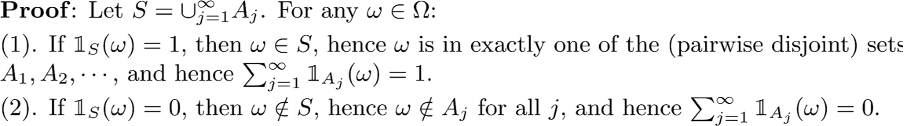
\includegraphics{Picture 1.png}
\caption{alt text here}
\end{figure}

\end{document}
